\documentclass[11pt,a4paper]{article}

% ---------- Packages ----------
\usepackage[utf8]{inputenc}
\usepackage[T1]{fontenc}
\usepackage{lmodern}
\usepackage{amsmath,amssymb}
\usepackage{enumitem}
\usepackage{geometry}
\usepackage{fancyhdr}
\usepackage[most]{tcolorbox}   % enhanced, breakable
\usepackage{hyperref}
\usepackage[siunitx]{circuitikz}

% ---------- Geometry ----------
\geometry{margin=2.5cm}

% ---------- Header/Footer ----------
\setlength{\headheight}{14pt}  % fancyhdr warning verhindern
\pagestyle{fancy}
\fancyhf{}
\lhead{Introduction to Electrical Engineering}
\cfoot{\thepage}

% ---------- Exercise Environment ----------
\newcounter{exercise}
\newenvironment{exercise}[1][]
  {\refstepcounter{exercise}%
   \begin{tcolorbox}[enhanced, breakable, width=\textwidth,
     colback=blue!5!white,colframe=blue!60!black,
     fonttitle=\bfseries\large,
     title=Exercise~\theexercise:~#1]}
  {\end{tcolorbox}}

% ---------- Solution Environment ----------
\newif\ifshowsolutions
\showsolutionstrue  % comment to hide solutions

\newenvironment{solution}
  {\ifshowsolutions
     \begin{tcolorbox}[enhanced, breakable, width=\textwidth,
       colback=green!5!white,colframe=green!50!black,
       fonttitle=\bfseries\large,
       title=Solution]}
  {\end{tcolorbox}\fi}

% ---------- Document ----------
\begin{document}

% ----- Header Box -----
\begin{tcolorbox}[enhanced, breakable, colback=gray!10!white,
  colframe=gray!70!black, fonttitle=\bfseries\large,
  title={Exercise Sheet \#2}, sharp corners, width=\textwidth]
\begin{center}
  DC 1
\end{center}
\end{tcolorbox}
\vspace{1cm}

% ----- Exercise 1 -----
\begin{exercise}[KCL]
Find  $i_1$, $i_2$, and $i_3$.

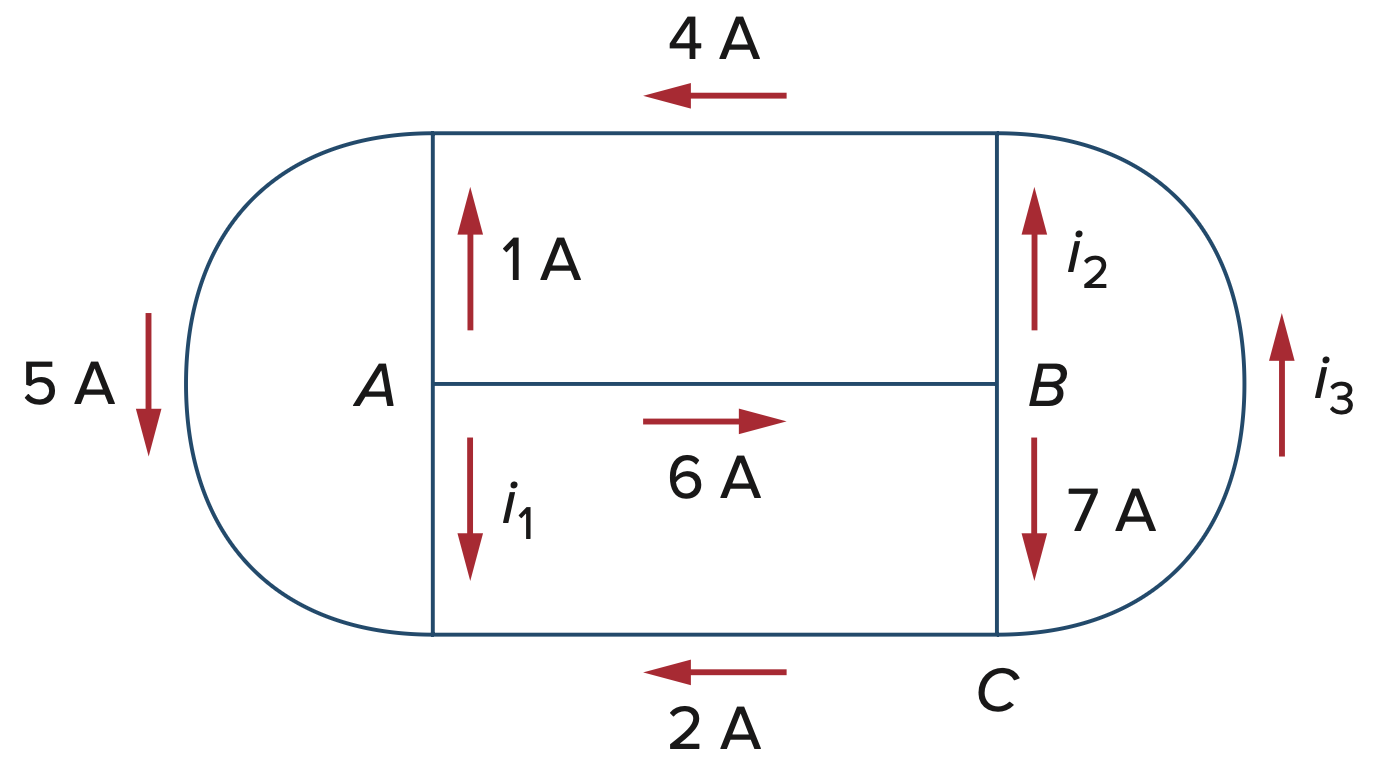
\includegraphics[width=0.7\textwidth]{figures/kcl.png}
\end{exercise}

\ifshowsolutions
\begin{solution}
node A:
\[
-1\, \mathrm{A} - 6\, \mathrm{A} - i_1 = 0
\]
\[
\Rightarrow i_1 = -1\, \mathrm{A} - 6\, \mathrm{A} = -7\, \mathrm{A}
\]

node B:
\[
6\, \mathrm{A} - 7\, \mathrm{A} - i_2 = 0
\]
\[
\Rightarrow i_2 = 6\, \mathrm{A} - 7\, \mathrm{A} = -1\, \mathrm{A}
\]

node C:
\[
7\, \mathrm{A} - 2\, \mathrm{A} - i_3 = 0
\]
\[
\Rightarrow i_3 =  7\, \mathrm{A} - 2\, \mathrm{A}= 5\, \mathrm{A}
\]

... other nodes:
\[
i_2 + i_3 - 4\, \mathrm{A} = 0
\]
\[
\Rightarrow i_2 = 4\, \mathrm{A} - i_3 = -1\, \mathrm{A}
\]
\end{solution}
\fi

% ----- Exercise 2 -----
\begin{exercise}[KVL]
Calculate  $V_1$ and $V_2$.

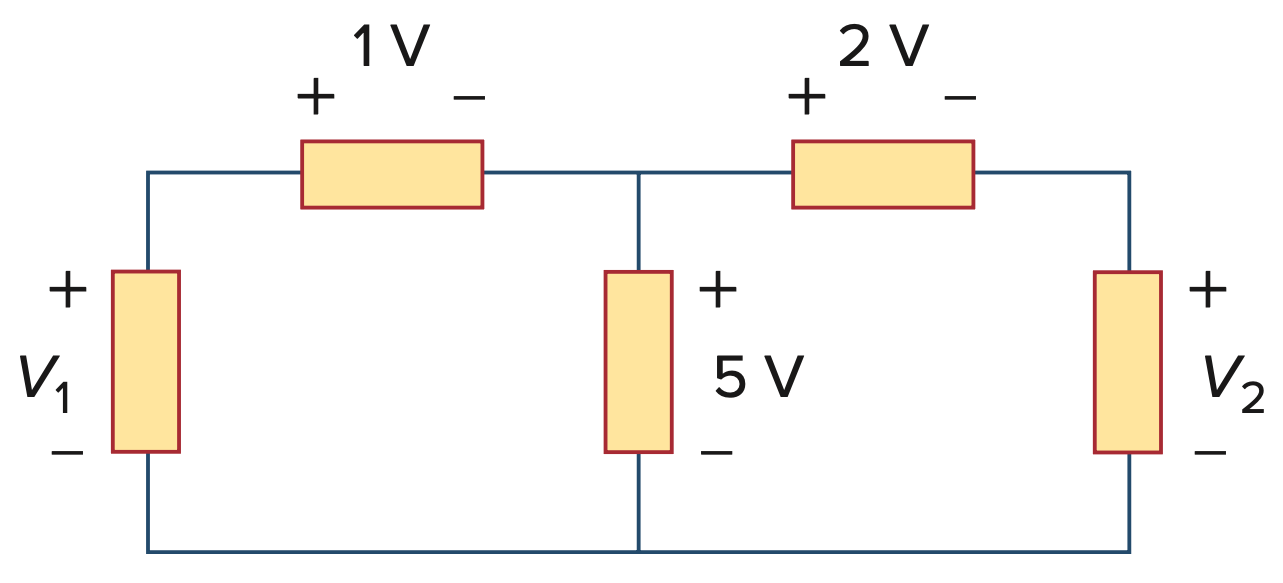
\includegraphics[width=0.7\textwidth]{figures/kvl.png}
\end{exercise}

\ifshowsolutions
\begin{solution}
\[
1\, \mathrm{V} + 5\, \mathrm{V} - V_1 = 0
\]
\[
\Rightarrow V_1 = 1\, \mathrm{V} + 5\, \mathrm{V} = 6\, \mathrm{V}
\]

\[
2\, \mathrm{V} + V_2 - 5\, \mathrm{V}= 0
\]
\[
\Rightarrow V_2 =  5\, \mathrm{V} - 2\, \mathrm{V}= 3\, \mathrm{V}
\]
\end{solution}
\fi

% ----- Exercise 3 -----
\begin{exercise}[Series and Parallel Resistors]
Calculate $I_0$.

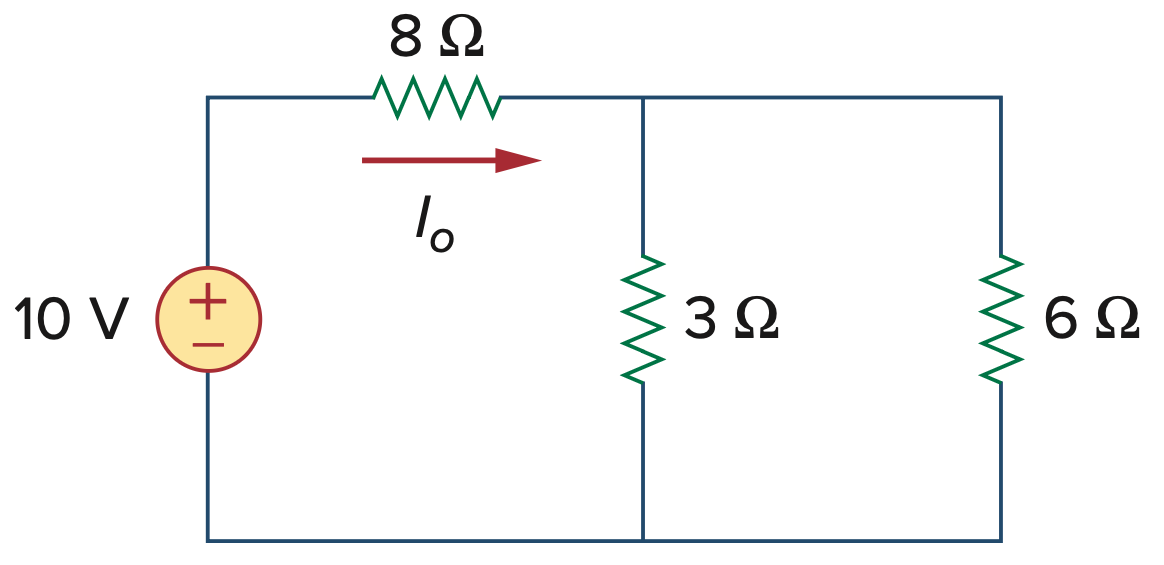
\includegraphics[width=0.7\textwidth]{figures/series_parallel.png}
\end{exercise}

\ifshowsolutions
\begin{solution}
First, we calculate the equivalent resistance of the parallel resistors with $3\, \Omega$ and $6\, \Omega$, then we add the series resistor with $8\, \Omega$:

\[
R = \frac{3\, \Omega \cdot 6\, \Omega}{3\, \Omega + 6\, \Omega} + 8\, \Omega= 10\, \Omega
\]

Finally, we can calculate the current \(I_0\) using Ohm's law:

\[
I_o = \frac{10\, \mathrm{V}}{10\, \Omega} = 1\, \mathrm{A}
\]
\end{solution}
\fi

% ----- Exercise 4 -----
\begin{exercise}[Series vs. Parallel]
Three light bulbs are connected in series to a $120\, \mathrm{V}$ source as shown below. Find the current $I$ through each of the bulbs. Each bulb is rated at $120\, \mathrm{V}$. How much power is each bulb absorbing? Do they generate much light?

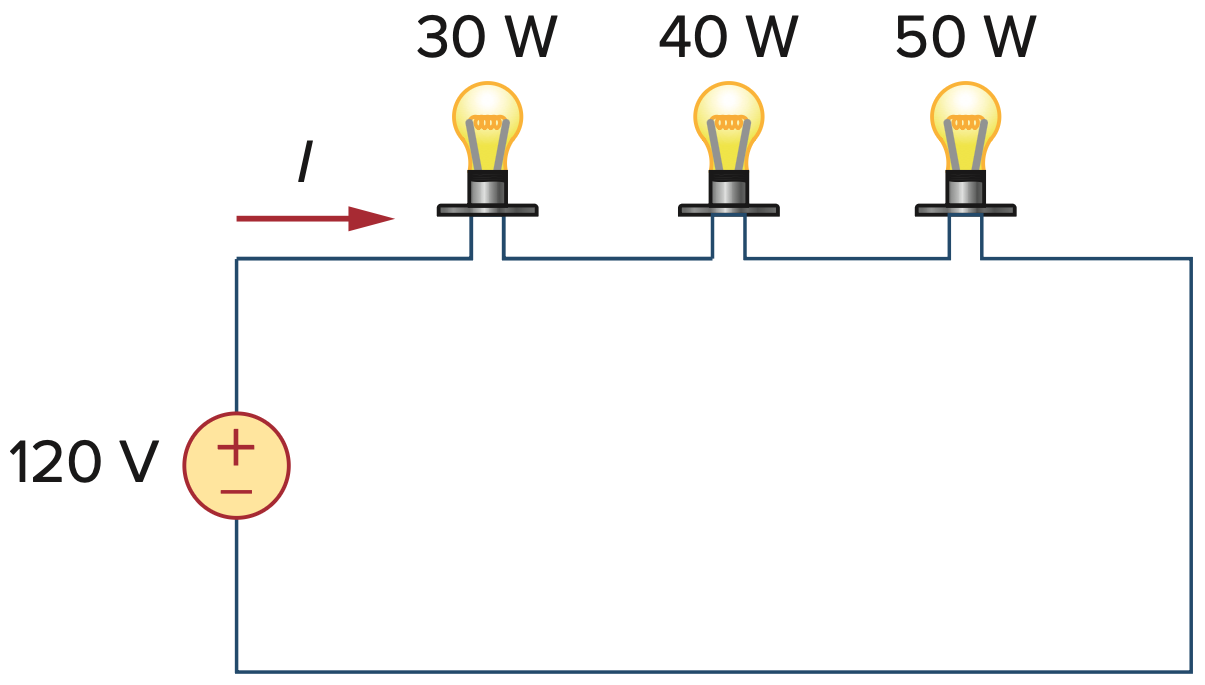
\includegraphics[width=0.7\textwidth]{figures/light_bulbs.png}
\end{exercise}

\ifshowsolutions
\begin{solution}
First, we calculate the resistances of each bulb using their rated power and voltage:
\[
R = \frac{V^2}{P}
\]

\[
R_{30\, \mathrm{W}} = \frac{(120\, \mathrm{V})^2}{30\, \mathrm{W}} = 480\, \Omega
\]

\[
R_{40\, \mathrm{W}} = \frac{(120\, \mathrm{V})^2}{40\, \mathrm{W}} = 360\, \Omega
\]

\[
R_{50\, \mathrm{W}} = \frac{(120\, \mathrm{V})^2}{50\, \mathrm{W}} = 288\, \Omega
\]

Then, we calculate the equivalent resistance of the three light bulbs in series:
\[
R = 480\, \Omega + 360\, \Omega + 288\, \Omega = 1128\, \Omega
\]

Then, we can calculate the current \(I\) using Ohm's law:
\[
I = \frac{120\, \mathrm{V}}{1128\, \Omega} = 0.1063\, \mathrm{A}
\]  

Finally, we can calculate the power absorbed by each bulb:
\[
P = I^2 \cdot R
\]

\[
P_{30\, \mathrm{W}} = (0.1063\, \mathrm{A})^2 \cdot 480\, \Omega = 5.432\, \mathrm{W}
\]

\[
P_{40\, \mathrm{W}} = (0.1063\, \mathrm{A})^2 \cdot 360\, \Omega = 4.074\, \mathrm{W}
\]

\[
P_{50\, \mathrm{W}} = (0.1063\, \mathrm{A})^2 \cdot 288\, \Omega = 3.259\, \mathrm{W}
\]

Clearly these values are well below the rated powers of each light bulb, so we would not expect very much light from any of them. To work properly, they need to be connected in parallel.
\end{solution}
\fi

% ----- Exercise 5 -----
\begin{exercise}[Equivalent Resistance 1]
Calculate the equivalent resistance $R_{ab}$ across the terminals.

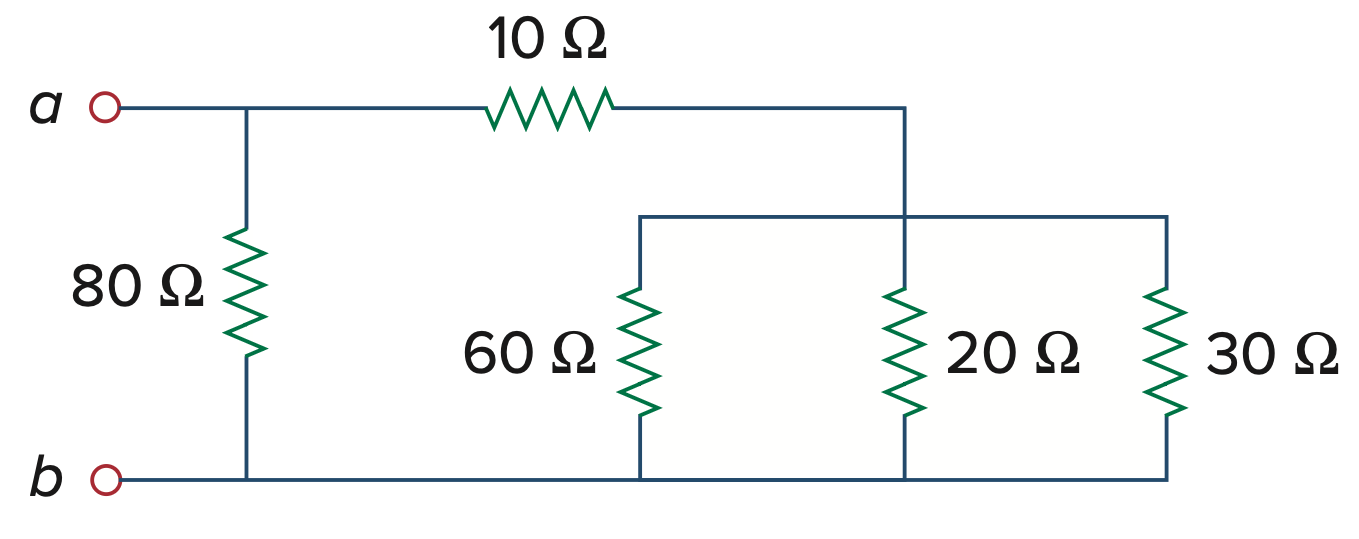
\includegraphics[width=0.7\textwidth]{figures/equivalent_R_1.png}
\end{exercise}

\ifshowsolutions
\begin{solution}
First we calculate the equivalent resistance of the parallel resistors with $60\, \Omega$, $20\, \Omega$, and $30\, \Omega$:
\[
R_p = \frac{1}{\frac{1}{60\, \Omega} + \frac{1}{20\, \Omega} + \frac{1}{30\, \Omega}} = 10\, \Omega
\]

Then we add the series resistor with $10\, \Omega$:
\[
R_{ab} = 10\, \Omega + 10\, \Omega = 20\, \Omega
\]

And finally we combine with the parallal resistor of $80\, \Omega$:
\[
R_{ab} = \frac{1}{\frac{1}{20\, \Omega} + \frac{1}{80\, \Omega}} = 16\, \Omega
\]
\end{solution}
\fi

% ----- Exercise 6 -----
\begin{exercise}[Equivalent Resistance 2]
Given the resistor network with $R_1 = 10\,\Omega$, $R_2 = 20\,\Omega$, $R_3 = 30\,\Omega$, $R_4 = 5\,\Omega$, $R_5 = 15\,\Omega$:

\begin{center}
\begin{circuitikz}[european, scale=1]

% Left terminal A
\draw (0,0) node[left]{A} -- (1,0);

% R1 in series
\draw (1,0) to[R=$R_1$] (3,0);

% Split node
\draw (3,0) -- (4,0);
\draw (4,0) -- (4,2);

% Upper branch: R2 and R3 in series
\draw (4,2) to[R=$R_2$] (6,2)
           to[R=$R_3$] (8,2)
           -- (8,0);

% Lower branch: R4
\draw (4,0) to[R=$R_4$] (8,0);

% Continue in series with R5
\draw (8,0) -- (9,0)
      to[R=$R_5$] (11,0)
      -- (12,0);

% Right terminal B
\draw (12,0) node[right]{B};

\end{circuitikz}
\end{center}

Calculate the equivalent resistance of the network between terminals A and B.
\end{exercise}

\ifshowsolutions
\begin{solution}
\[
R_{23} = R_2 + R_3 = 20 + 30 = 50\,\Omega
\]
\[
\frac{1}{R_{234}} = \frac{1}{R_{23}} + \frac{1}{R_4} = \frac{1}{50} + \frac{1}{5} = \frac{11}{50}\,\frac{1}{\Omega}
\]
\[
R = R_1 + R_{234} + R_5 = 10 + \frac{50}{11} + 15 = 29.55\,\Omega
\]
\end{solution}
\fi

% ----- Exercise 7 -----
\begin{exercise}[Current Divider Rule]
Calculate $i_1$ to $i_5$.

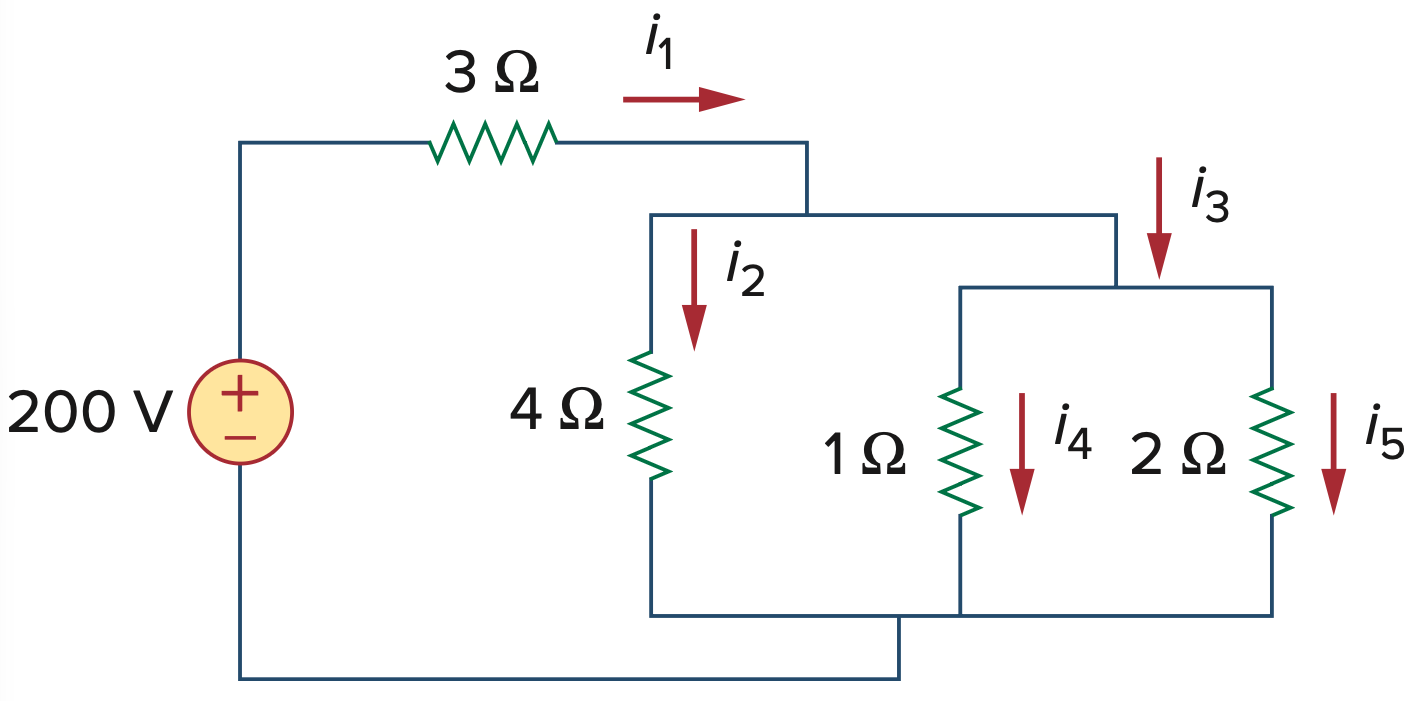
\includegraphics[width=0.7\textwidth]{figures/current_divider.png}
\end{exercise}

\ifshowsolutions
\begin{solution}
First, we calculate the equivalent resistance of the parallel resistors with $1\, \Omega$ and $2\, \Omega$ and call it \(R_3\):

\[
R_3 = \frac{1\, \Omega \cdot 2\, \Omega}{1\, \Omega + 2\, \Omega} = \frac{2}{3}\, \Omega
\]

Then we calculate the total resistance \(R\) from the $4\, \Omega$ resistor parallel to \(R_3\) and the $3\, \Omega$ resistor in series:

\[
R = 3\, \Omega + \frac{4\, \Omega \cdot \frac{2}{3}\, \Omega}{4\, \Omega + \frac{2}{3}\, \Omega} = \frac{25}{7}\, \Omega
\]

Using Ohm's law, we can calculate the total current \(i_1\):

\[
i_1 = \frac{200\, \mathrm{V}}{\frac{25}{7}\, \Omega} = 56\, \mathrm{A}
\]

Then, we can calculate \(i_2\) using current division:

\[
i_2 = i_1 \cdot \frac{R_3}{R_2 + R_3} = 56\, \mathrm{A} \cdot \frac{\frac{2}{3}\, \Omega}{4\, \Omega + \frac{2}{3}\, \Omega} = 8\, \mathrm{A}
\]

KCL gives us \(i_3\):

\[
i_3 = i_1 - i_2 = 56\, \mathrm{A} - 8\, \mathrm{A} = 48\, \mathrm{A}
\]

Again, we can calculate \(i_4\) using current division:

\[
i_4 = i_3 \cdot \frac{R_5}{R_4 + R_5} = 48\, \mathrm{A} \cdot \frac{2\, \Omega}{1\, \Omega + 2\, \Omega} = 32\, \mathrm{A}
\]

Finally, KCL gives us \(i_5\):

\[
i_5 = i_3 - i_4 = 48\, \mathrm{A} - 32\, \mathrm{A} = 16\, \mathrm{A}
\]
\end{solution}
\fi

% ----- Exercise 8 -----
\begin{exercise}[Circuit Analysis]
Calculate the equivalent resistance across the terminals.

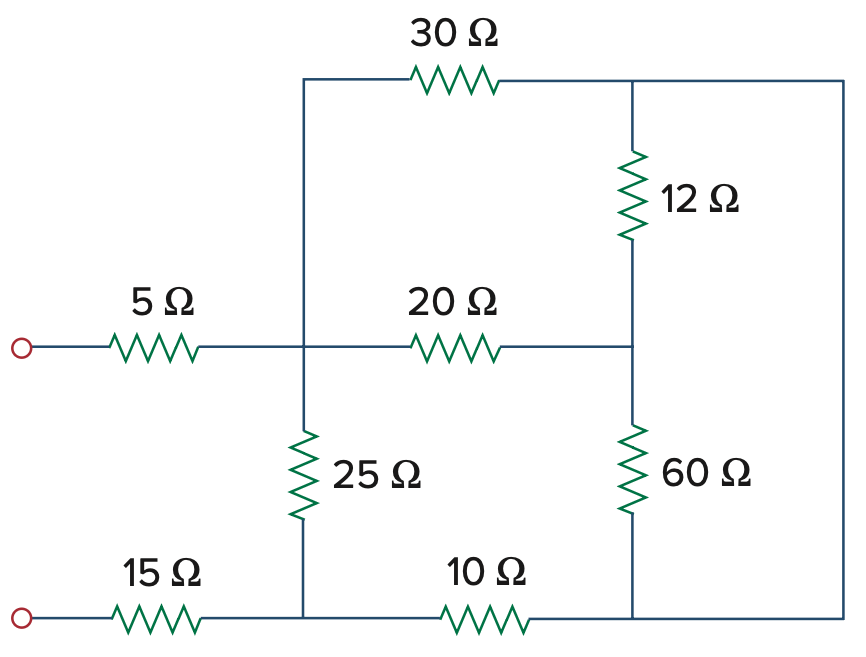
\includegraphics[width=0.7\textwidth]{figures/equivalent_R_2.png}
\end{exercise}

\ifshowsolutions
\begin{solution}
1. Combine the right vertical resistors:
\[
12\, \Omega \parallel 60\, \Omega = \frac{12\, \Omega \cdot 60\, \Omega}{12\, \Omega + 60\, \Omega} = 10\, \Omega
\]

2. Series combination with the $20\, \Omega$ resistor:
\[
20\, \Omega + 10\, \Omega = 30\, \Omega
\]

3. Parallel combination with the other $30\, \Omega$:
\[
30\, \Omega \parallel 30\, \Omega = \frac{30\, \Omega \cdot 30\, \Omega}{30\, \Omega + 30\, \Omega} = 15\, \Omega
\]

After these three steps, the circuit reduces to a triangle ($\Delta$):

\begin{center}
\begin{circuitikz}[american]
    \draw
    (0,0) node[anchor=east]{}
    to[R=$15\,\Omega$, o-*] (2,0)
    to[short] (3,0)
    to[R=$10\,\Omega$] (5,0)
    node[circle,draw,fill=white,inner sep=1pt,label=below:$N_3$]{};

    \node[circle,draw,fill=black,inner sep=1pt,label=above:$N_1$] (N1) at (2,4) {};
    \node[circle,draw,fill=black,inner sep=1pt,label=below:$N_2$] (N2) at (2,0) {};

    \draw
    (0,4) node[anchor=east]{}
    to[R=$5\,\Omega$, o-*] (2,4)
    to[R=$25\,\Omega$] (2,0)
    (2,4) to[R=$15\,\Omega$] (5,0);
\end{circuitikz}
\end{center}

4. Convert the $\Delta$-network to equivalent Y-resistances:
\[
R_1 = \frac{R_b R_c}{R_a + R_b + R_c} = \frac{15\, \Omega \cdot 25\, \Omega}{50\, \Omega} = 7.5\, \Omega
\]
\[
R_2 = \frac{R_a R_c}{R_a + R_b + R_c} = \frac{10\, \Omega \cdot 25\, \Omega}{50\, \Omega} = 5\, \Omega
\]
\[
R_3 = \frac{R_a R_b}{R_a + R_b + R_c} = \frac{10\, \Omega \cdot 15\, \Omega}{50\, \Omega} = 3\, \Omega
\]

\begin{center}
\begin{circuitikz}[american]
    % Nodes
    \node[] (A) at (0,4) {};
    \node[] (B) at (0,0) {};
    \node[circle,draw,fill=white,inner sep=1pt,label=above:$N_1$] (N1) at (2,3) {};
    \node[circle,draw,fill=white,inner sep=1pt,label=below:$N_2$] (N2) at (2,1) {};
    \node[circle,draw,fill=white,inner sep=1pt,label=right:$N_3$] (N3) at (5,2) {};
    \node[circle,draw,fill=white,inner sep=1pt] (O) at (3.5,2) {}; % star center

    % External connections
    \draw (A) to[R=$5\,\Omega$, o-*] (N1);
    \draw (B) to[R=$15\,\Omega$, o-*] (N2);

    % Star (Y) arms
    \draw (O) to[R=$7.5\,\Omega$] (N1);
    \draw (O) to[R=$5\,\Omega$] (N2);
    \draw (O) to[R=$3\,\Omega$] (N3);

\end{circuitikz}
\end{center}

The branch with the \( 3\, \Omega \) resistor connects to a dead-end node \( N_3 \), so it carries no current and can be ignored.
\[
\Rightarrow R_{eq} = 5\, \Omega + 7.5\, \Omega + 5\, \Omega + 15\, \Omega = 32.5\, \Omega
\]

Alternative for 4. without $\Delta$-Y transformation:

Since $N_3$ is a trivial node (just one input and one equal output), you can simply calculate the series resistance of the $15\, \Omega$ and $10\, \Omega$ resistors, then combine it in parallel with the $25\, \Omega$ resistor, and finally add the series resistors with $5\, \Omega$ and $15\, \Omega$.
\end{solution}
\fi

\end{document}